\documentclass[tikz,border=2pt]{standalone}
\usepackage{pgfplots}\pgfplotsset{compat=1.17}
\usepackage{helvet}\renewcommand{\familydefault}{\sfdefault}
\begin{document}
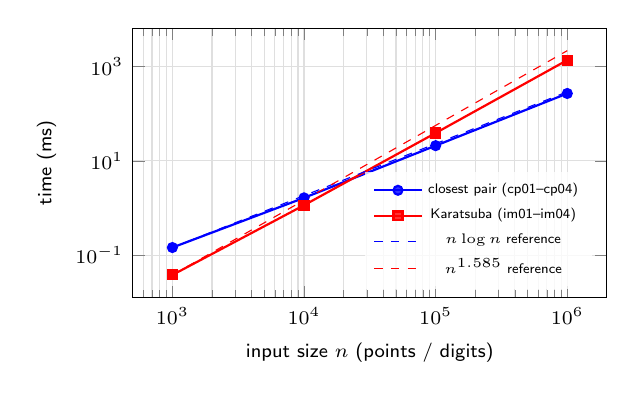
\begin{tikzpicture}
\begin{axis}[width=7.6cm,height=5.0cm,xmode=log,ymode=log,
  xlabel={input size $n$ (points / digits)},ylabel={time (ms)},
  tick label style={font=\scriptsize},label style={font=\scriptsize},
  legend style={font=\tiny,at={(0.97,0.03)},anchor=south east,draw=none,fill=white,fill opacity=0.8,text opacity=1},
  grid=both,grid style={gray!25},mark size=1.6pt]
\addplot[blue,mark=*,thick] coordinates {(1000,0.145)(10000,1.638)(100000,20.924)(1000000,267.319)};
\addlegendentry{closest pair (cp01--cp04)}
\addplot[red,mark=square*,thick] coordinates {(1000,0.038)(10000,1.144)(100000,38.839)(1000000,1361.753)};
\addlegendentry{Karatsuba (im01--im04)}
\addplot[blue,dashed,domain=1000:1000000,samples=2] {0.145*(x/1000)*ln(x)/ln(1000)};
\addlegendentry{$n\log n$ reference}
\addplot[red,dashed,domain=1000:1000000,samples=2] {0.038*(x/1000)^1.585};
\addlegendentry{$n^{1.585}$ reference}
\end{axis}
\end{tikzpicture}
\end{document}
